% Created 2018-07-15 Sun 12:39
% Intended LaTeX compiler: pdflatex
\documentclass[11pt]{article}
\usepackage{graphicx}
\usepackage{grffile}
\usepackage{longtable}
\usepackage{wrapfig}
\usepackage{rotating}
\usepackage[normalem]{ulem}
\usepackage{amsmath}
\usepackage{textcomp}
\usepackage{amssymb}
\usepackage{capt-of}
\usepackage{hyperref}
\usepackage{fontspec}
\setmainfont[BoldFont={Gentium Basic Bold}, ItalicFont={Gentium Basic Italic}]{Gentium Plus}
\usepackage{polyglossia}
\setmainlanguage{english}
\setotherlanguage{hebrew}
\newfontfamily\hebrewfont{SBL Hebrew}
\usepackage[margin=0.8in]{geometry}
\author{Steven Tammen}
\date{June 24, 2018}
\title{Teaching the Ancients to Type: Better Unicode Text Entry for Ancient Greek and Hebrew}
\hypersetup{
 pdfauthor={Steven Tammen},
 pdftitle={Teaching the Ancients to Type: Better Unicode Text Entry for Ancient Greek and Hebrew},
 pdfkeywords={},
 pdfsubject={},
 pdfcreator={Emacs 25.3.1 (Org mode 9.1.13)}, 
 pdflang={English}}
\begin{document}

\maketitle
\setcounter{tocdepth}{2}
\tableofcontents



\section{Section 1: What is this project? Why this project? Why this paper?}
\label{sec:orgd2f1b44}

\subsection{What is this project?}
\label{sec:org651c2d6}

While this project has many different goals and subgoals (and continues to add more as additional matters of convenience and usability come up), the essential aim is to create easy-to-use keyboard layouts for \emph{non-native} languages. What exactly does this mean?

Typists for a particular language can usually be classified rather easily into native speakers and non-native speakers. Native speakers type their language "a lot" -- with respect to both frequency and quantity -- while non-native speakers do not. For example, someone who is bilingual in English and Spanish might type approximately 50\% of their text in either language; they have two native languages. However, someone who types 90\% of their text in English and 10\% in German (perhaps to communicate with a colleague or business associate) has only one native language -- English. The lines can get blurry, of course, but the general idea is that one can usually cleanly categorize languages based on how often and how long they are typed: some are typed often and for a long time (native languages), and others are not (non-native languages).\footnote{This is admittedly not exactly how native and non-native languages are typically defined, but hopefully it is a forgivable simplification. People who type a language they did not grow up speaking as a significant percentage of their total volume may not be "native speakers" by some people's definitions, but the terminology is employed here for the purpose of avoiding such verbose titles as "effectively native languages" and "non-effectively native languages."}

In theory, keyboard layouts for native languages should be designed according to certain keyboard design metrics that make typing more efficient. Nowadays, optimization is accomplished through computer programs that change letters in a configuration until additional changes do not improve the layout any more. Such an approach is known as a \emph{genetic algorithm}. Examples of this approach may be seen for Chinese in Liao and Choe (2013) and for Arabic in Malas, Taifour, and Abandah (2008).\footnote{People interested in this process are encouraged to visit \url{http://www.adnw.de}. This site contains much background on the history of keyboard layout optimization, and a well-documented C++ optimizer program. The main focus of this site is German layouts, but there is a fair bit of discussion for English layouts as well.}

Layouts designed in this manner perform better with respect to typing metrics such as low overall hand movement (which helps reduce unnecessary movement away from the home row) and high hand alternation (which helps prevent many characters from getting typed contiguously by one hand while the other sits idle). However, since different languages have different frequently used phonetic patterns/letter combinations, so-called "optimal" layouts for different native languages will place even phonetically and orthographically identical letters in very different places.

The question of whether or not it is better for bilingual and trilingual (etc.) individuals to try and learn one keyboard layout that is a compromise between their multiple languages or separate keyboard layouts for each language is a fascinating one, but it is ultimately separate from the matters this project concerns itself with. This project is instead focused on situations of language imbalance -- given that there is a dominant keyboard layout (presumably for one's native language), what is the best way to type non-native languages?

\subsection{Why this project?}
\label{sec:orgd6c5465}

Multilingual text input for non-native languages is a solved problem. By this I mean that at the time of writing, it is possible with various existing software options to enter text both in a primary language and in multiple alternate scripts (e.g., Greek, Hebrew, Cyrillic, Arabic, Devanagari) with relative ease.

So why bother working on another project addressing these things? It's a fair question.

\subsubsection{To combat the lack of open source, \emph{customizable} software}
\label{sec:org7a1974d}

This section will use the present state of Greek text input as an example to illustrate how customizable software is currently lacking. Similar situations and observations hold for other languages that I have knowledge of, but will not be discussed for brevity's sake.\footnote{Discussion of options from research in Hebrew. Maybe put in Appendix somewhere?} \\

\noindent \textbf{Current options for Greek text input} \\

\{Todo: discussion of various already existing software options. List from Bibliography, explicit coverage of system options.\} \\

\noindent \textbf{Positive characteristics} \\

Among different options one can observe several important design characteristics. Some (which? be specific) solutions are \emph{homophonic}, meaning that alpha is put on the A key, beta on the B key, and so forth. Some (which? be specific) attempt to avoid complex chord sequences when entering diacritical marks by using punctuation-based mnemonics. Some (which? be specific) allow flexible entry order, meaning that breathing-then-accent or accent-then-breathing (for example) both correctly display. Many (which? be specific) allow for text entry across applications rather than having to copy and paste out of some "special" window. All of these things are definite positives for a typist, especially one switching into Greek text entry from time to time while primarily typing in his/her native language(s). \\

\noindent \textbf{Customization and open source} \\

However, users who wish to customize things are out of luck with present options. Some people may wish to change how diacritics are handled, for example, or to change which Latin-script letter chi goes on to conform to their preferences (both C and X are popular, but it is irritating to have to deal with both mappings). Because current options are closed source without significant customization interfaces, this is simply not possible.

Customization and open source software go hand-in-glove, and especially for a program such as this -- which is dealing with a very domain-specific problem that contains much that is subjective and/or related to user preference -- there is significant benefit to making software community-driven. 

Of course, open source software has some other benefits as well. Open source software is free and relatively more stable than close sourced software. There is never a guarantee of long-term stability with programs that do not publish their source code, since if the projects stop getting maintained (a company goes out of business, e.g., or the primary developer dies suddenly), nobody else can pick them up and keep the code running smoothly on new hardware and/or operating system environments. This is actually a somewhat greater concern for projects of this sort: since programs dealing with keyboard layouts must depend on system calls to interface with keyboards, they are necessarily less insulated from the operating system environment than many other kinds of programs. In other words, if an operating system changes one of its low-level libraries for handling streams of keys, it will likely break a program dealing with keyboard layouts, while a browser or music player might still work just fine.

If I were forced to pick "just one" reason why this project existed, it would be this: to create a customizable and open source framework for text entry of non-native languages.

\subsubsection{To combat the lack of software that bundles multiple language layouts together}
\label{sec:org7fa2698}

This software is being developed in close association with Classicists, and the initial project scope is, in many ways, targeted at solving the problems of Greek scholars in this field. However, I am trying to create a framework that may be comfortably extended to other languages and alphabets as needed.

Some academic fields (e.g., Historical Linguistics, Classics, Ancient Near East, and Ancient History), have significant language demands. It is not uncommon for people studying in these fields to pick up multiple ancient languages (including, but certainly not limited to, Latin, Greek, Hebrew, Arabic, Syriac, and Sanskrit), with many of these having complex alphabets. A lack of consistency in approaches can be frustrating, particularly if one has to go through the bother of installing and updating text entry solutions for all these languages on all the computers used for writing.

Additionally, much secondary scholarship in these fields is in German, French, and Italian, all of which share the basic English character set, but demand a few special characters and/or accents. It is conceivable for a scholar working on research about Mediterranean trade in Late Antiquity, for example, to need to type in English for their core analysis, Latin, Greek, and Syriac for primary sources, and German, French, and Italian for secondary sources. Assuming Latin is typed without macrons and accents, that leaves 5 additional languages on top of English that must be dealt with.

While it is more a future goal than a priority of "round one" of this project, bringing multiple language layouts together in the same program is one of the central motivations behind creating another project dealing with these things. Starting from scratch rather than adding on to an existing program ensures that there will be seamless interoperability in the future, and that standards and design guidelines may be established.

\subsubsection{To combat the lack of software that adds functionality without removing any}
\label{sec:org188886b}

Using keyboard shortcuts can be a frustrating experience when you have to type in another language. If there is no intelligent handling of modifier keys, people typing in a non-native language might miss such shortcuts as Ctrl-C (copy), Ctrl-X (cut), Ctrl-V (paste), Ctrl-Z (undo), and Ctrl-S (save). The situation is especially bad for those who use Vim, Emacs, or other text editors that make use of the keyboard (rather than a GUI) for functionality, and for people who use keyboard-driven window managers, browsers, application launchers, window switchers, and so on.

It can also be frustrating to "lose access" to some English keys (typically punctuation such as brackets) when typing in another language. If a language layer "steals" English punctuation keys thinking that they will never be needed when typing that language, but does not provide any way to access said keys short of disabling the software temporarily, it can create an unpleasant user experience.

Things like these are not the most obvious design factors when one thinks of typing in non-native languages, but it has been my experience that these are actually almost as important as the layout design itself. The devil truly is in the details.

\subsubsection{To combat the lack of software that works for nonstandard keyboard layouts}
\label{sec:orgafb369f}

Another reason for the creation of this project in particular is the fact that currently available homophonic layouts (at least those that function at the system level) do not work for "nonstandard" keyboard layouts -- they all assume a QWERTY base mapping.

People typing on Dvorak, Colemak, QWERTZ, BÉPO, and so forth may wish to have the benefits of homophonic letter layouts in their non-native languages while retaining their native base mapping. Portability is a high priority of this project, and all of the functionality in any language can be implemented on whatever base layout is desired, with full customization as an option.

\subsection{Why this paper?}
\label{sec:org29fe62c}

\subsubsection{Justifying design choices}
\label{sec:org215e827}

This paper is intended to fill the void between low level implementation details (should arrays or strings be used to send keys? Global variables or classes?) and the end result of fully functioning keyboard layouts.

I personally find it extremely frustrating when design decisions have no specific thought process behind them. For this reason I am attempting to document things in such a way that I would be satisfied as a user of this software, if I were not the one designing it in the first place. The placement of letter keys, the choice of particular punctuation keys for diacritics, the mechanism for switching languages, the process of entering "normal" punctuation when on a non-native layer; these are the sorts of design decisions that this paper sets out to explain.

The idea is to have something to point to when someone asks, "but why?" Rather than saying "just because" or trying to come up with rationalizations \emph{ex post facto}, attempting to rigorously justify everything from the get-go should lead to a project wherein there are not an abundance of arbitrary program characteristics. At least in theory.

\subsubsection{Creating a starting point for people that may have different opinions than myself}
\label{sec:org1f1d065}

With all this being said, this paper is certainly not attempting to close discussion on these topics or be the last word on design factors. At the time of writing, I have worked with Greek for approximately two years, and any sort of serious coding for about as long. I am sure one could easily find people more qualified than myself for virtually any aspect of this project, and also for all of them put together.

Instead, the idea is start a conversation about these things in a more formal manner. I am certain that Classicists, for example, are opinionated about how they wish to type Greek, and things that drive them crazy about current options that let them type Greek. If this paper can present one rationale that can be critiqued and examined, and the code behind this project is designed in such a way that it is sufficiently flexible, it should be possible in the future for this project to come to encompass multiple points of view, and circle in on an increasingly sophisticated understanding of the design variables in play.

\{Todo: maybe mention survey and results here?\}

\section{Section 2: Nuts and bolts}
\label{sec:org382642d}

Before getting into this project in particular, it is proper to briefly examine the nuts and bolts that make multilingual text input a possibility on modern operating systems. Much more could be written about any of the things here, but the present section will seek only to provide a sufficient amount of background to give readers an appreciation for the complexity at play behind the scenes.

\subsection{Keyboard layouts}
\label{sec:orgf3504d8}

To be able to type in a language that is not the default for your physical keyboard and system layout (e.g., a QWERTY ANSI keyboard used for American English), a different keyboard layout is necessary. In essence, a keyboard layout translates presses of physical keys into characters or key events (like Enter or Tab).\footnote{To be more precise, keyboards send signals that are interpreted by the operating system. Depending on permissions, different programs can inject themselves into the input system, and intercept keypresses before they get sent to other programs. This is what allows a remapping program to change the behavior of sent keys: the signals sent by the physical keyboard are the same, but they are intercepted and replaced with so-called "virtual keys" that lead to different behavior.} I find it helpful to split up keyboard layouts for languages into smaller semantic groupings to make them easier to think about, especially for people that must implement them in software.

\subsubsection{Letters}
\label{sec:org786e601}

For languages with alphabets (\{Todo: footnote: as opposed to syllabaries or Abjads\}), keyboard layouts must provide a means for typing all of the letters. English has 26 letters, but other languages often have more or less.

Letters may be further subdivided into vowels and consonants. Vowels are typically the more interesting variety inasmuch as most markup (such as accents) revolves around vowels, and therefore they typically require more work to integrate into the layout. For example, Greek vowels may take accents, breathings, iota subscripts, and so forth, while Greek consonants (with the exception of rho) take none of these things. This means that designers do not need to keep track of consonants as closely as vowels, generally speaking.

Many languages have uppercase and lowercase letterforms, but not all languages do. Hebrew, for example, does not have any casing distinctions. In general, implementing uppercase forms involves keeping track of shift state, but not too much extra work other than that.

\subsubsection{Context-specific/alternate letter forms}
\label{sec:orgfbb2dbb}

Some languages have letters that change their form based upon their position in words. For example, word-final sigma in Greek changes forms, and many letters in Hebrew and Arabic also exhibit this behavior.

Semantically, the letter is still the same, and should not therefore be thought of as a new or different entity. However, implementing positional letterforms does require some extra work, particularly in terms of identifying word boundaries. One approach to handling final forms is replacing the base form with the final form when and only when a key signifying a word boundary (such as Space or .,?!) is pressed immediately following a letter with final form behavior.

In addition to final forms, some languages have alternate forms of letters. In Hebrew, for example, some of the so-called Begadkephat letters (tav, dalet, gimel) have alternate forms for when they are aspirated, while others (bet, khaf) fully change their phonetic value through an alternate form. The line here can be a bit blurred between these alternate forms (which use a mark called a \emph{dagesh}) and letters with diacritics. The dagesh can be used with other Hebrew consonants to double phonetic value, for example, which could be considered a separate use. But the same mark is used.

For simplicity in programming, I recommend structuring development around \emph{program features} (for example, the ability add a dagesh to things\ldots{} alternate form or no) rather than \emph{language features} (for example, working on developing the capacity to support all possible sounds in a language, including aspirated forms and those that optionally change their phonetic value). This allows the designer of a keyboard layout to focus on one thing at a time, rather than trying to organize development around language features that may not cleanly map onto structured commits. As long as pains are taken not to forget any essential language features, this approach is easier on the programmers while accomplishing the same goals.

\subsubsection{Mandatory markup: accents, vowel points, etc.}
\label{sec:org0884770}

Most languages have some system of diacritical marks that are considered mandatory, diacritical marks that are essentially "part of the language." For example, Spanish and Italian have accents, Hebrew has vowel points, and Greek has accents, breathing marks, and the iota subscript.

These mandatory diacritical marks must be present for language text to be considered correct, and are often used frequently. For this reason, they require more thought in placement, since an inconvenient location or entry method can render text entry for the entire language unpleasant.

\subsubsection{Additional markup: vowel quantity, cantillation marks, etc.}
\label{sec:org074c3c0}

Some languages have another set of markup symbols used in specific circumstances or by specific groups of people. Good examples of symbols in this category are diacritics that indicate vowel quantity: the macron and breve are not "required" in Latin-script languages, but commonly show up in dictionaries and grammar books to help with pronunciation.

There are also other domain-specific symbols, depending on the language. Hebrew scholars working with the Masoretic text in any capacity will inevitably have to deal with the cantillation marks (the \texthebrew{טעמי המקרא}, \emph{ta'amei ha-mikra}), used in ritual chanting of the Tanakh. Greek and Latin scholars may wish to use metrical symbols to mark dactyls, spondees, and caesurae when scanning ancient epics in dactylic hexameter. Etc.

Implementation of these additional markup symbols is in some sense optional, inasmuch as they are used only by certain groups of people. However, it is best to think of them as features that should be included eventually for robustness, even if they do not make it into the first implementation.

\subsubsection{Punctuation; language-specific symbols}
\label{sec:orgf511e20}

While the dominance of English as a computer language has served to standardize international punctuation to a certain extent, some languages still have specific punctuation that is used in lieu of, say, the question mark. Greek, for example, uses a semicolon to indicate questions, and a dot in the middle of the line to indicate a break in thought (i.e., to indicate a semicolon).

The situation is somewhat complex in that "casual typing" of many languages has led to a situation in which punctuation systems are mixed. It is not uncommon to see Greek imperatives followed by exclamation points in introductory texts, for example, even though this has no precedent in ancient sources.

Numerals are another interesting case. Arabic numerals (0-9) are very much the international standard nowadays, but many languages used to use different numerical systems with different character sets (sometimes some subset of the alphabet, as with Hebrew), which may have special numerical symbols.

Finally, in modern contexts, most foreign currencies have special symbols. It is convenient to be able to access these without complicated and abstruse key sequences or combinations.

\subsection{Unicode}
\label{sec:org667025f}

\subsubsection{History}
\label{sec:org8592bbf}

Handling languages with non-Latin alphabets has long been a topic of conversation among people working with computer input systems. Due to historical reasons, computers have developed very much around English and the ASCII character set, with other alphabets being second class citizens.

As computers developed and people moved away from typewriters (which had significant physical limitations that made representing many complex scripts difficult), efforts were undertaken to standardize language input and robustly handle foreign alphabets, even their mixing with English. For example, Knisbacher et al. (1989) discuss Hebrew input on early PCs, and Selden (1981) summarizes an early effort to standardize how Arabic was handled on computers.

However, early systems suffered from problems that made them somewhat less than optimal: many systems made it impossible to mix English and a foreign text, foreign text typed in one system often was not portable to other systems, etc. Mastronarde (2008) discusses such problems in the first few pages of his discussion of pre-Unicode options for Greek input.

As memory and storage sizes have increased, it has become acceptable to use multiple bytes for the storage of text characters, and thus much easier to handle all of the characters necessary for multiple complex alphabets. Unicode attempts to solve the challenges of dealing with multiple languages by defining values that map to characters across different numeric ranges. In this way, Unicode allows for multiple languages to be typed without conflict, since the characters are all being represented by different numbers in memory.

\subsubsection{Scope and purpose; peculiarities}
\label{sec:orge088aa2}

Unicode is theoretically laid out in terms of "blocks" for different language sections. Unfortunately, due to various considerations (politics, lack of foresight, an initial project scope that did not encompass historical/uncommon characters), it is not uncommon for characters of the same language to be spread out across several numerical ranges. The initial Greek block, for example is sufficient for monotonic Greek accentuation, but leaves a lot to be desired in terms of polytonic Greek. The Greek extended block helps in the area of polytonic Greek, but still leaves many uncommon or regional characters without official support.

Unicode seeks, in some sense, to be the "kitchen-sink" solution. When you type Unicode text in a document with encoding such as UTF-8, you have the capability of using all of the 1-million-plus characters together (a decidedly good thing). However, the nature of its all-encompassing haphazard growth has made it somewhat more difficult to understand from a language-centric perspective (e.g., you are using two or three of the hundreds of possible languages, and have no need for the rest), and has caused the full encoding to include some puzzling, kludgy behavior.

A good resource discussing such Unicode peculiarities from the Greek side of things is Nick Nicholas' page on Greek and Unicode: \url{http://www.opoudjis.net/unicode/unicode.html}. Many Unicode choices that seem strange at first glance may still seem strange at second glance too, but typically there are reasons for why things are the way they are (even if they are unsatisfying and historical).

\subsubsection{Precomposed and decomposed Unicode}
\label{sec:org2591c2c}

As time has passed, the Unicode consortium has gotten more and more reserved about adding additional precomposed characters. After all, so the reasoning goes, combining diacritical marks are already supported in the Unicode specification. Why should Unicode have to support "redundant" precomposed characters if you can just enter the same character as a sequence with combining characters?

The logic is fine so far as it goes, but the problem is that the Unicode text encoding is only half of the picture: without fonts that properly support decomposed sequences, decomposed Unicode is not really an option. There have historically been many problems with fonts improperly displaying combining characters. For example:

\begin{itemize}
\item The combining characters might be horizontally off-center compared to the letter
\item The vertical spacing between the letter and the diacritic might be too little or too much
\item Multiple combining characters might overlap with each other, or not stack properly
\item Etc.
\end{itemize}

Because different base characters have different physical characteristics (e.g., some are taller or wider or have ascenders and descenders to deal with) there is no cookie-cutter solution for physically placing combining characters. Rather, it must be done for each letter individually.

As will be discussed below, there are actually modern fonts that handle decomposed Unicode well. However, there are still plenty of fonts that do not, especially when you start combining multiple diacritics, or using any uncommon diacritics.

\subsubsection{Combining multiple diacritics}
\label{sec:orgc125784}

An additional wrinkle in decomposed Unicode with multiple combining characters is the entry sequence. What happens if you type all the permutations of three different diacritics -- do they all display the same?

The answer will typically be no. In the second chapter of the Unicode 11 manual (\url{http://www.unicode.org/versions/Unicode11.0.0/ch02.pdf}), section 11 deals with combining characters, and discusses the default combining behavior for multiple combining characters:

\begin{quote}
By default, the diacritics or other combining characters are positioned from the base character’s glyph outward. Combining characters placed above a base character will be stacked vertically, starting with the first encountered in the logical store and continuing for as many marks above as are required by the character codes following the base character. For combining characters placed below a base character, the situation is reversed, with the combining characters
starting from the base character and stacking downward.
\end{quote}

Because some languages violate the expected behavior due to historical reasons, it is usually safest to check how a particular language typically handles the entry order of combining characters. An example of such a resource for Greek comes from the Greek and Unicode site linked above: \url{http://www.opoudjis.net/unicode/unicode\_ordering.html}.

\subsection{Fonts}
\label{sec:org9d80be1}

\subsubsection{Supporting decomposed Unicode}
\label{sec:org30055c1}

In recent years, font support for decomposed Unicode has improved significantly. In particular, support for so-called "smart fonts" (such as OpenType fonts) has improved to the point where most users will not have to concern themselves about whether or not their fonts play nice with decomposed Unicode so long as they are using popular mainstream fonts (Lucida Grande, Palatino Linotype) or common academic fonts for their language(s).\footnote{See \url{https://gervatoshav.blogspot.com/2015/07/greek-fonts-free-productivity-apps-and.html} and \url{http://www.russellcottrell.com/greek/fonts.asp} for good discussions of Greek options, and \url{https://jcuenod.github.io/bibletech/2017/07/27/unicode-hebrew-fonts/} for a good discussion of Hebrew options. Domain specific fonts (such as the SBL fonts) will not support as wide a range of characters -- the IPA blocks, for example -- as more general fonts that have broad coverage (such as Cardo).} Mastronarde (2008), on pages 26-28, includes a good discussion of how fonts behave with smart features vs. how they behave without smart features, and has a helpful chart illustrating why smart features are to be desired. Of course, this is somewhat an application problem as well, since if an application does not support OTF fonts, for example, it will not support decomposed Unicode either (or at least is likely to not display it cleanly). Fortunately, most modern text processing applications support smart fonts just fine, and so this is more of an academic concern than a practical concern.

With all this having been said, even smart fonts can fail to handle some of the less common combinations. Macrons prove problematic in many otherwise excellent Greek fonts, for example, since there are not precomposed forms for combinations like macron + acute accent, and since decomposed macron + accent forms do not always display nicely. The path to fixing such problems is not always clear (since it might require the coordination of font designers, input system developers, and the developers of word-processing software), but usually there is a way.\footnote{A good example of font changes that can be undertaken to solve such problems can be seen in a series of blog posts by James Tauber, starting with this post: \url{https://jktauber.com/2016/01/28/polytonic-greek-unicode-is-still-not-perfect/}}

\subsubsection{Private Use Areas}
\label{sec:orgd704543}

One very straightforward way of handling edge cases is to create special precomposed characters for them so that combining character stacking never even comes into the picture. Unicode supports the use of so-called "private use areas" (PUAs)-- ranges of Unicode codepoints (E000 - F8FF and planes 15 and 16) that are purposely left undefined by Unicode to allow for organizations/other groups to create non-standard character definitions. A good FAQ on the characters defined in these ranges ("private use characters") can be found on the Unicode website: \url{https://www.unicode.org/faq/private\_use.html}.

The technical details section of the GreekKeys site (\url{http://apagreekkeys.org/technicalDetails.html}) discusses the use of PUAs for special Greek characters by a collection of Unicode fonts including GreekKeys's New Athena Unicode, Juan-José Marcos' Alphabetum, David Perry's Cardo, and others. The page also includes a link to  Juan-José Marcos' proposal for the agreement: \url{http://apagreekkeys.org/pdfs/PUA\_coordination\_usage.pdf}. This pseudo-standard allows for many characters Unicode does not directly support to be typed by Greek scholars who wish to use them. New Athena Unicode also supports some additional characters in the PUAs (as mentioned in the above link) that the other fonts may not.

If you are willing to only view and publish documents with fonts that follow such "gentlemen's agreements" for PUA characters, you may find solutions like this to be extremely useful. However, using PUA points is not at all portable, since if someone were to open your document with a font that did not define the PUA code points (or perhaps even worse, defined them with entirely different characters), your text would not display correctly.

\subsubsection{Using the same font for native languages and non-native languages}
\label{sec:org45b8228}

One final thing to note about fonts is their interaction with publishing systems. Depending on your particular application choices (e.g., Microsoft Word, \LaTeX{}, InDesign), it may or may not be possible to have custom font faces on a per-language basis. That is, without any additional work on your part, can you have text in, e.g., Greek, show up on screen and print in an entirely different font than the English text?

An argument in favor of certain workflows is the customization options they give you. For example, I currently write in Emacs' Org mode, and export to PDF via \LaTeX{}. I can tell Emacs to use different fonts depending on the character set (to have my preferred fonts on screen when I am writing in foreign scripts), and tell \LaTeX{} to use entirely different fonts for different languages when publishing, all without having to manually change fonts every time I switch a language.

However, for most people, setting up something like the above is a big headache. It is easy, however, to use a Unicode font that supports multiple character sets, including, for example, the Latin character block and the Greek blocks. Writing in a font like Cardo, New Athena Unicode, Gentium Plus, SBL BibLit, etc. lets you write both English and Greek without having to change fonts, and works this way no matter what application you use the font in, as long as said application supports Unicode. The broader support a particular font has, the more different languages you can type in that font without having to worry about font switching.

\section{Section 3: The Unicode Language Layers project}
\label{sec:orgfae844a}

Thus far we have examined exactly what this project is interested in at a high level (§1), and the sorts of details that must be dealt with when working with multilingual input on computers (§2). This section will seek to present a brief summary of this project's main goals and features.

\subsection{Sane defaults combined with ease of use}
\label{sec:org6d254bd}

A popular sentiment in the programming community is the notion of having software that "just works." Equally prevalent is the notion that software should follow the "principle of least astonishment."\footnote{Interested parties may learn about what these phrases at \url{http://wiki.c2.com/?ItJustWorks} and \url{http://wiki.c2.com/?PrincipleOfLeastAstonishment}.} The former refers to the idea that software should be \emph{easy} (for normal humans) to download, install, run, update, and what have you. If grandma needs to open bash and pipe a man page through grep to find out how to resize a window, software does not just work. The latter refers to the idea that software should behave according to how (normal humans) would expect it to behave. Software that has a button with an X on it that opens a new window is not following the principle of least astonishment.

These desirable traits are bandied about quite a bit, but, it seems to me, less common in software than one might think. This project seeks to both "just work" and be predictable as much as possible, given the limitations on my time and present programming capabilities.

\subsubsection{Installing and running the program}
\label{sec:orgdabdca3}

Aside from installing a language dependency (AutoHotkey), which is unfortunately unavoidable, installing and running this project is very straightforward. You download the zip file containing the program, unzip it, and double click on the remapping program to run it.

Assuming you are using QWERTY, you do \emph{not} have to change anything about your current keyboard, operating system keyboard layout, word processing software, and so on. If you are not using QWERTY, see §3.2, below.

You do not need to touch any system configuration like Control Panel, and the program is portable (as long as you have AutoHotkey, which can also be installed portably -- see the zip file on \url{https://www.autohotkey.com/download/})

\subsubsection{Intuitive switching between languages}
\label{sec:orgae27f7c}

Depending on what sort of software you use for typing in other languages, you may need to go into the system tray to switch languages, or select between possible layout options with a shortcut like Win + Space (the Windows key plus Space). Key sequences are desirable when switching between languages since they don't force you to reach for a mouse and open some different window.

In particular, it is useful to be able to switch to specific languages with key sequences, rather than toggling between multiple options. If you need to type in more than two scripts, having a single keyboard shortcut may force you to press a sequence multiple times to select the language you really want (cf. the normal behavior of Alt + Tab). It is more efficient (and arguably easier to remember) to have separate hotkeys for changing to desired languages individually (a hotkey to start typing in English, a hotkey to start typing in Greek, a hotkey to start typing in Hebrew, etc.). It is even better if these individual sequences use mnemonics for memorability. 

This is the approach taken by this project. Currently, CapsLock serves as what I call the "language leader key" -- when you press it, the next key has special behavior associated with language functionality. To switch between languages, all you need to do is remember the mnemonics:

\begin{itemize}
\item CapsLock + e = switch to English mode
\item CapsLock + g = switch to Greek mode
\item CapsLock + h = switch to Hebrew mode
\end{itemize}

\subsubsection{Letter placements that make sense}
\label{sec:org30bc71b}

Since this project is targeting the typing of non-native languages (see §1.1), letter placements should be intuitive for typists that are not typing in a language frequently or for a long time. \\

\noindent \textbf{Typing performance and keyboard layout considerations} \\

Studies of typing have identified some trends in terms of keystroke efficiency and general typing performance. For example, Dhakal \emph{et al.} (2018), in a study of 168,000 volunteer typists, found that inter-key intervals (IKIs) -- the time intervals between subsequent key presses, a good predictor of overall typing speed -- were lower for bigrams (two-letter sequences) that alternated hands (i.e., had one letter typed by one hand, and a following letter typed by the other hand) than for bigrams typed on only one hand. Feit \emph{et al.} (2016), in their overview of previous studies of typing, summarize well established phenomena and their corresponding measures based on prior studies of professional touch typists; the finding reported above has been noted multiple times in prior studies. Additionally, it has been observed that repeated key presses have lower IKIs than same-hand key presses (with keys pressed by different fingers), which in turn have lower IKIs than keypresses that require the same finger to press two different keys in succession.

Dhakal \emph{et. al} (2018) also found that faster typists make/need to correct fewer mistakes than slower typists, that faster typists use more fingers on average, and that faster typists have high "rollover percentages" -- a measurement of how many keystrokes begin with other keys already being pressed down from a previous keystroke. Feit \emph{et al.} (2016) observed a similar phenomenon in that they came to the conclusion that the preparation of keystrokes leads to lower average IKIs. They also noted that a lower standard deviation in global hand position (i.e., lower overall hand movement from some "home position") similarly leads to lower average IKIs, and that a consistent key mapping of finger-to-key ("low entropy") has a similar effect.

Pulling these observations together, one arrives at something like the following:

\begin{itemize}
\item Bigrams involving hand alternation are faster (in terms of low IKIs) than repeated keypresses (i.e., a bigram with only one unique key pressed twice by the same finger), which in turn are faster than (non-same-finger) same-hand bigrams, which in turn are faster than (non-repeated) same-finger bigrams.
\item The ability to "prepare" following keypresses positively associates with typing speed (low IKIs), which helps explain why fast typists have high rollover percentages: lining up future keystrokes makes it easier for fast typists to have multiple keys down at the same time.
\item Low overall hand movement positively associates with typing speed (low IKIs). This is likely mediated through low-movement typists being better able to line up future keypresses.
\item The number of fingers used to type positively associates with typing speed (words per minute: WPM).
\item A low error rate positively associates with typing speed (WPM).
\item A consistent mapping of finger-to-key ("low entropy") positively associates with typing speed (low IKIs).
\end{itemize}

Mapping these observations onto keyboard layout design is not exactly 1:1. The above studies had populations of almost entirely QWERTY typists. QWERTY heavily loads the left hand, and does not actually favor a neutral hand position on the home row since very frequent letters such as e, t, r, o, i, n, etc. are not actually on the home row. (This would have the net effect of actually \emph{penalizing} people that learned a 10-finger touch typing system that teaches slavish hand positioning on the home row). Moreover, the second study did not have any typists above 79 words per minute, which is below the \emph{average} 80+ WPM typing rates of earlier studies that focused on trained, professional touch typists (on typewriters, no less, which disallow rollover by mechanical design). For these reasons, I do not agree with the conclusion of this study that touch-typists (defined as people able to type without looking at the keyboard to find keys) and non-touch-typists have similar typing speeds on a philosophical level: perhaps for the suboptimal QWERTY layout for typists of slow to average speeds, but not in general, and almost certainly not for typists on right tail of the distribution, with speeds exceeding 120 WPM. In other words, while I do think that the study is valuable in that it shows that most average typists won't benefit from a structured system, I do not think it says anything about the usefulness of the structured system as one approaches higher speeds, particularly on more intentionally designed keyboard layouts.\footnote{Full disclosure: I type on an algorithmically generated custom layout (with heavy automation built in: autospacing of punctuation, autopairing of parentheses etc., autocapitalization, and so forth), and have spent a great deal of time over the years thinking about these things. See \url{https://github.com/StevenTammen/hieam}.}

Additionally, it is somewhat difficult to map things like "low error rate" onto keyboard layouts. Perhaps some keys are more easy to confuse than others, and some sequences of keypresses are harder on a physiological level, but these things are difficult to measure, and may vary widely by individual.

With all this being said, present data does support prioritizing bigram hand alternation, prioritizing low overall hand motion, and minimizing the amount of consecutive non-repeat keypresses involving the same-finger. \\

\noindent \textbf{The design of non-native keyboard layouts} \\

Given the above discussion, one might wonder if it is worth designing keyboard layouts for non-native language that try to minimize IKIs and maximize WPM by their very design. Once in muscle-memory, they would certainly allow for higher theoretical speeds.

However, the exceedingly great complexity of the cognitive processes behind typing -- see Rumelhart \emph{et al.} (1982), e.g., for a specific proposed model-- makes it difficult to pin down performance causalities, particularly with respect to mental models of keyboard layouts. For example: what effect do semantic groupings of characters have?

As a general rule of thumb, so-called "fully optimized" layouts (which tend to have high hand alternation, low overall hand movement, and low same-finger) will have relatively poor inherent memorability in terms of semantic groups. If you let a genetic algorithm design an optimized layout for you, it will not keep all the letters in a block or numbers in a row, but mix everything together according to frequency considerations. We humans are very pattern-oriented creatures, and having no apparent structure to characters will inevitably make a keyboard layout more difficult to remember, to some degree. Furthermore, it would seem likely that keyboard layouts that are easier to remember will be easier to get up to speed with, especially if you don't practice with them very much.

The issue in all this is that there is no research I am aware of that explicitly covers these things. For this reason, I cannot say definitely how much easier semantically-grouped keyboard layouts for non-native languages are to learn than fully-optimized keyboard layouts for these same languages, or how much faster people may train them to, say, 35 WPM. The data for this simply does not exist. However, this paper is operating on the assumption that these considerations are non-negligible for most people in most circumstances. The hypothesis coming from such an assumption is this: since people typing non-native languages will not be typing them with great frequency and magnitude, it is more rational to focus on memorability over raw optimization considerations, since layouts that are easier to remember will be faster to learn, and the benefits of "brute forcing" an optimized layout (as one might do for one's native language) will never be realized in typical use cases. \\

\noindent \textbf{Native-language layouts in muscle memory} \\

The above discussion focused on the interplay of memorability, layout optimality (as measured by hand alternation, overall hand movement, same-finger, etc.), and ease of acquisition in the abstract. However, assuming users of this project can already type on a keyboard layout in their own language (in whatever regard: touch typing, hunting and pecking, etc.), we do not need to start from ground-zero.

The general idea is that for the circumstances under which most people type non-native languages it is \emph{always} better to associate a keyboard layout for a non-native language with a keyboard layout for a native language already in muscle memory. Associating a new layout with the old layout lets typists reuse neural pathways that are already in place rather than forming new ones from scratch.

What do I mean by this? Let's take the Greek letter alpha. Most people, Classicists or no, know that alpha corresponds in phonetic value to the English letter A. Alpha also happens to look like the letter A in both its lowercase and uppercase forms. So, rather than putting alpha on some random key, why not simply place it on the same key as the letter A in English? \\

\noindent \textbf{Issues in constructing associations} \\

If we accept the premise that it is best to form correspondences between non-native languages and keyboard layouts already in use (for English or otherwise), then it follows that we need some formalized system for doing so.

Layouts derived from phonetic matching are typically called "homophonic layouts." While homophonic layouts are excellent when correspondences exist, there are some letters in languages that have no clear English equivalent. Theta in Greek, for example, corresponds to the phoneme in English that is represented by the digraph "th." These must be dealt with separately.

There are also some cases when a language has two letters for the same phoneme. In Hebrew, for example, the consonant vet (bet without a dagesh) is equivalent to the consonant vav -- they both make "the V sound." So which one should occupy the V key?

The associations (henceforth keymaps, short for "key mappings") in §4.1 and §5.1 below attempt to solve such issues in a systematic way. Following the hypothesis presented above (namely, that memorability is a more important concern in these circumstances than raw optimality), priority is given to phonetic correspondences, then visual correspondences, then transcription correspondences, then, finally, to raw optimality.

The ordering of priority above is not based on any hard data (as no such data exists, to my knowledge), but based on my own experiences in learning Greek and Hebrew keyboard layouts, the principle of least astonishment, and logical consistency:

\begin{enumerate}
\item Following the principle of least astonishment, if "most" keys are being placed by phonetic correspondence, it makes sense to use phonetic correspondence as the primary determiner of non-native character position, wherever possible.
\item Following this, visual correspondences are used since they do not depend on any particular system (unlike transcription correspondences, which may only "work" for some transcription schemes), and also have greater "astonishment factor" for alternate keymaps than transcription correspondences (particularly in the case of Greek, which shares many graphemes with English in lowercase and especially uppercase forms). For example, eta in Greek is almost universally put on the letter H in keyboard layouts, since capital eta \emph{is} the grapheme H.
\item Transcription correspondences come next, in that they are a better mnemonic than nothing. Transcription correspondences work best for letter-based transcription (i.e., transcription that does not involve the used of special diacritics), especially that involving only single graphemes. A good example of this is using Q for quf on Hebrew keyboard layouts: the English letter Q most certainly does not take on the phonetic value [k], but since quf is very commonly transliterated as Q, it is easy to associate the letter Q with quf.
\item Finally, raw optimality is used when none of the mnemonics work. The letter theta in Greek, for example, has no phonetic \emph{letter} equivalent in English (even though we use the phoneme \emph{θ} all the time), has no letter look-alikes, and is commonly transliterated as th or tʰ, which doesn't help create any good associations (since tau makes the most sense for the English letter T). So theta is placed on a key that performs best with respect to the goals of high hand alternation, low overall hand movement, and low same-finger.
\end{enumerate}

\subsubsection{Diacritic placements that make sense}
\label{sec:org0c129a6}

Since diacritics don't have phonetic value or any transcription equivalencies most of the time, finding memorable places for them relies much more on visual correspondences and raw optimality. The visual correspondences here are a little less obvious as well (e.g., : yields a diaeresis as apposed to a yields α).

This is one of the key areas that this project distinguishes itself from others. Many (but not all) keyboard layouts for languages like Greek and Hebrew use either dead-keys or complicated chords (Ctrl + Alt/Option + something) to enter diacritics, which is far harder to remember than a single key equivalence, particularly a key equivalence with visual correspondence. Single keys (even those that require shift to enter) are also much faster to type in general.

As with letters, visual correspondences are prioritized above raw optimality, following the same hypothesis that memorability is of greater concern for the keyboard layouts of non-native languages than theoretical measures of efficiency.

\subsubsection{Diacritics that just work}
\label{sec:orgd25f42b}

Unicode diacritics can be implemented in such a way that adding and removing them becomes complex and messy. For example:

\begin{itemize}
\item If precomposed Unicode is entered with stateless key combinations, adding or removing a diacritic to a letter that has already been typed involves deleting the entire last character and then pressing a new (correct) key combination.
\item If diacritics are entered by means of decomposed Unicode, display problems commonly occur if diacritics are entered in an incorrect order. For example, if a user types alpha then an acute accent, and then, a couple second later, decides that that alpha should also have a macron, he or she typically \emph{cannot} just press the diacritic key for the macron: due to how Unicode treats multiple combining characters (see §2.2.4), the accent will appear closer to the alpha than the macron, which is typically not the stacking behavior that is desired.
\item If diacritics are entered by means of decomposed Unicode, by default there is no way to change or remove diacritics any way but sequentially. That is, if you have something like alpha + smooth breathing + circumflex + iota subscript, and wish to either remove the smooth breathing or change it to rough breathing, you will have to delete all three diacritics to be able to change the breathing.
\item Etc.
\end{itemize}

This project abstracts \emph{all} of the messy implementation details away from the user. In this project, diacritics are added to a letter by pressing the \emph{single} keys associated with them, typically linked mnemonically (see §3.1.4, above). They can be added in any order, but will always display correctly. They can also be removed in any order: pressing a diacritic key again when the diacritic is already on the preceding letter will remove it, \emph{no matter where it is}. Whether it was the last combining character entered or three back, it will still get removed while leaving all the other diacritics untouched. Finally, changing between options within a diacritic category that has mutually exclusive choices does not require deleting an old option before switching to a new option (although it still works seamlessly if you choose to do it this way). So, for example, if you had typed our sequence from above, alpha + smooth breathing + circumflex + iota subscript, but wanted to change that circumflex into an acute accent, all you would need to do is press the diacritic key for the acute accent. The circumflex would get deleted automatically, and replaced with an acute accent.

For many keyboard layouts, if a user wants to be able to enter both precomposed and decomposed Unicode, he or she may need to learn two entirely different systems of entering diacritics. Moreover, if software does not provide any mechanism for switching Unicode output type, a user may not even have the ability to choose. This project lets users choose between precomposed and decomposed Unicode, and handles entry in exactly the same way. That is to say, how you add and remove diacritics (as described above) is consistent for both precomposed and decomposed Unicode, so you can freely switch between them without having to worry about different systems of entry.

One final thing: the logic used by this project is smart enough to use precomposed Unicode all they way up to the point it is not supported, and then switch to decomposed Unicode on the fly. If you are typing with the Unicode send type set to precomposed, entering alpha + acute will lead to a precomposed character getting sent, but pressing the key for a macron after this will lead to three characters getting sent (decomposed Unicode), since there are no precomposed forms for macrons with accents. (At least not in the Unicode base specification that is supported by this project at this time; PUA code points are different matter).

\subsubsection{Intuitive backspacing behavior}
\label{sec:org25daaeb}

When typing normal text, the Backspace key deletes the last character; this is what people expect it to do. However, unless handled by software, when combining characters are used in decomposed Unicode, Backspace will only delete the last diacritic. Not only is this surprising for people who have never had to deal with it before, but it also makes backspacing full vowels inconvenient.

This project enables the use of Backspace as one would use it normally: pressing Backspace once deletes one letter, regardless of the number of diacritics attached to said letter. Removing individual diacritics (see the section immediately preceding this) is still possible, but is accomplished by pressing the diacritic key for the already-present diacritic that you wish to remove.

\subsubsection{Quiet error checking and handling}
\label{sec:org13d8ef9}

This project attempts to catch and handle errors as they happen. If when adding a diacritic you would enter an illegal diacritic combination (in Greek, epsilon or omicron + circumflex, e.g.), the program simply acts as if you had never pressed the offending diacritic key: the state of the program is reset to be exactly as it was before the new key was pressed. Depending on the diacritics in question, the program will also automatically overwrite mutually exclusive diacritics (e.g., a macron and a circumflex for Greek vowels -- a circumflex indicates a vowel is long, making a macron unnecessary), so that there is a never a circumstance in which you add both to a letter, then get surprised when you remove one only to find the other present even though it wasn't showing before. This makes the diacritics fully "what you see is what you get" (WYSIWYG): you will never have to face a situation in which there are diacritics associated with a letter (through the program state) that are not currently showing.

Additionally, if you try and enter an illegal key sequence with the language leader key (e.g., in the present implementation, something like CapsLock + Space), the program will simply exit the language leader state and act as if nothing happened.

The benefit of doing these things is that it minimizes the amount of extra work you have to do if you realize you've done something wrong, and prevents unexpected behavior. If such handling was not present, you might, for example:

\begin{itemize}
\item Try to add a diaeresis to an iota with rough breathing, only to have it come back and act strangely later. Since the diaeresis is never word initial in Greek (being used to indicate that a successive vowel is pronounced separately rather than as a diphthong), and rough breathing is always word initial, this combination is not valid. But if it were not handled appropriately, it would be possible to either enter it as if it were valid (bad), or show only the rough breathing or diaeresis but not both, even though both would be present in the program logic, and would show if the other were removed (also bad). The only way to avoid "surprising" behavior is to simply "eat" the keypress of a diacritic if it would lead to an invalid combination.
\item Accidentally type CapsLock + r (currently undefined), intending instead to type CapsLock + e (switch to English mode). If you typed a g after this (thinking you were in English mode), and no error-handling had been done, you would instead switch to Greek mode since you would have never left the language leader state, and CapsLock + g switches to Greek mode.
\item Etc.
\end{itemize}

This sort of thing admittedly isn't perfect (what if you realized you pressed CapsLock + r instead of CapsLock + e \emph{before} you typed something else? Now due to the error handling you have to press CapsLock again before you can press e to switch to English), but it does seek to minimize the amount of "surprising" behavior that occurs, in line with the principle of least astonishment.

\subsubsection{Areas that need work}
\label{sec:org563d023}

This project is still very young, and I am still inexperienced as a programmer, objectively speaking. Moreover, the time constraints on this project have forced a focus on "central features" over less essential but more user-targeted features. Thus, while I hope it is clear from the above discussion that time has been spent trying to design a program that has a good default configuration and is easy to use,
there are still many areas where this project falls short of what it could be. I have collected a list of the most important features (in no particular order) that would improve the project with regards to default behavior and ease of use. It is hard to say how many of these will ever be implemented, but on a philosophical level, they would make the project better in these areas.

\begin{enumerate}
\item A more effortless installation and updating process. This might include offering an installer that packages AutoHotkey directly with the project code, and automatically extracts everything. The installer could also allow for the creation of a desktop icon and start menu shortcut, give the option of starting the program upon system startup (so that it would never need to be run manually), and automatically check for program updates.
\item More zero-setup default layer choices. For example, supporting Dvorak, Colemak, QWERTZ, AZERTY, and BÉPO out of the box.
\item Supporting the PUA Greek codepoints (see §2.3.2) for things like precomposed macrons with accents, epsilons and omicrons with circumflexes, and so forth. This would give wider default Greek support for more usage edge cases.
\item On the fly customization of settings with control sequences (hotstrings). For example setting the Unicode send type with a key sequence like \texttt{\textbackslash{}precomposed\{Enter\}} or \texttt{\textbackslash{}decomposed\{Enter\}} instead of having to update it through a config file or menu.
\item On-screen keyboard graphics for the currently active keyboard layout and layer. For an example of what this might look like, see the \href{http://pkl.sourceforge.net/}{Portable Keyboard Layout} project.\footnote{A reasonable introduction to this program can be found here: \url{https://www.makeuseof.com/tag/learn-keyboard-layout-portable-keyboard-layout/}. This page also includes a picture of what one of the persistent on-screen layouts looks like.} If not this, it would be helpful to at least have some visual indicator of what language you are currently in.
\item GUI customization of program options (as opposed to editing the config file by hand, which some users may find intimidating).
\item GUI customization of keyboard layouts/language layers, as opposed to having to deal with the code directly for changing things.
\item If possible to implement in a program-agnostic way (i.e., separate from some specific text-editor or word-processing application), supporting diacritic and backspacing behavior regardless of location in a text field. Currently you cannot move to a previously typed letter and add diacritics to it, for example.\footnote{This is a whole lot less trivial to implement than first meets the eye. Most programs that let you change diacritics on the fly have some way to access the file/text object you are working on directly (i.e., have read/write permissions for the file on disk and have it open through the kernel, or have some equivalent mechanism on the web). However, such programs are not portable; you cannot go back and dynamically change diacritics if you are typing in an email client, for example, since the text box in the email client is not in the special environment that enables the file checking (lookbehind) necessary for on the fly diacritics and backspacing.} If not possible, at least supporting a backspacing buffer to maintain intelligent backspacing for longer intervals than single characters, which is all that is currently supported.
\end{enumerate}

\subsection{Customizability as a first order priority}
\label{sec:org0cb3de8}

As mentioned in §1.2.1, one of the big reasons why this project has been undertaken is because current options, while they are not so much lacking in basic functionality, \emph{are} lacking in customization options, particularly customization options that:

\begin{enumerate}
\item Allow virtually everything about non-native language keyboard layouts to be changed, rather than just a few select things.
\item Expose the actual code so that motivated users can tailor things exactly to their liking without being crippled by not fully understanding how the implementation works.
\item Have thorough documentation.
\end{enumerate}

Taking these things in order:

\subsubsection{Full control}
\label{sec:org5e77d28}

Since this project is little more than a base script defining what happens when you press a specific key, it is possible to change \emph{everything} about the layout. You can change which keys do what, what special functions are called (such as those handling diacritics and modifiers) and when, and what language layers are used for each key.

Since the script does not have to deal with most of the runtime logic explicitly (e.g., the main loop listening for key presses and interpreting them is handled by the AutoHotkey language itself), it is safe to change the behavior of individual keys without worrying about breaking everything. Care has been taking when writing the code to keep keys isolated from each other so that changing the behavior of one individual key will not interfere with other keys.

In particular, it is possible to change the locations of all letters and diacritics for each language separately. This allows for a very fine level of control.

\subsubsection{Open source}
\label{sec:org7648e9d}

Assuming you are motivated enough to dive into the code, you \emph{can} do virtually whatever you want with the base that is provided. If you don't like how things are done, in large or small part, you can change it.

\subsubsection{Documentation}
\label{sec:orgb15558b}

Of course, the ability to change things is somewhat wasted if modification is made so difficult that only programming geniuses can understand the code so as to effectively make use of it. To some extent, there is no way to make most customization "drag and drop,"\footnote{Well, this would be the idea behind the GUI customization of layouts/layers mentioned in §3.1.8. The thing is, creating something that allows for somewhat-automatic customization is a monumental effort that requires programmatic code generation and a great deal of logic that has nothing to do with essential remapping functionality. Which is why it was not even considered for inclusion in the first round of this research project.} but pains have been taken in this project to make it as straightforward as possible. In particular:

\begin{enumerate}
\item There is a section in the program's Readme about customizing variables that were judged to be subjective to such a degree that easy customization was deemed important. This would include things like what language the script starts in, and whether the Unicode sent is precomposed or decomposed.
\item There is an API in the repository \{Todo: complete + link\} that documents the functions provided (both general functions and language specific functions), and includes examples of how customize various facets of program behavior.
\item There is a guide in the repository \{Todo: complete + link\} that covers the creation of remapping scripts for different base keyboard layouts. Aside from this, the already completed QWERTY remapping script provides a working example that may be used to help design new remapping scripts.
\item There is also a guide in the repository \{Todo: complete + link\} that covers the creation of new language layers and how to effectively integrate them with an already-existing remapping script. Best practices and soft design standards are also discussed in this document. Aside from this, the already-completed Greek and Hebrew layers (and the global constants and functions that accompany the layers) provide working examples that may be used to help design new non-native keyboard layouts.
\item The code itself is documented with in-line comments, and tries to follow good programming practices -- such as using meaningful variable names and avoiding the use of unnamed constants ("magic numbers") -- to make it self-documenting. Most of the functionality in this program is not especially difficult conceptually, and the whole project is split into layers to make customization as straightforward as possible.\footnote{As opposed to avoiding function-call overhead and writing everything in big methods for each key that are much harder to conceptualize and change in bulk.}
\end{enumerate}

\subsection{Minimal interference with normal computer use}
\label{sec:orgb9b6863}

To use a specific example, having the ability type in Greek is very useful for those of us who are Classicists. But it is a whole let less useful if it is difficult to activate the Greek keyboard and/or switch back to English when done typing Greek; if you can't use normal keyboard shortcuts when typing in Greek, that is no good either. These usability issues are arguably just as important for keyboard layouts as the letter layouts, if not more so.

\subsubsection{Quick and easy on and off}
\label{sec:org6aecd71}

As mentioned in §3.1.2, this project uses simple key sequences to switch between languages. Avoiding complex and hard to remember key sequences means this implementation does not get in the way of writing, even when switching between languages very frequently. If you are in fact switching between languages a lot (e.g., you are writing some sort of lexicon, or dealing with English descriptions of non-native phrases) the benefits will be more noticeable than if you are typing longer blocks in a non-native language less often.

\subsubsection{Consistent keyboard shortcuts}
\label{sec:org4c106f4}

Most people are familiar with and use keyboard shortcuts like Ctrl-C, Ctrl-X, Ctrl-V, Ctrl-Z, and so on. Losing these when you are typing in a non-native language can be supremely irritating.

To be fair, it is possible to make keyboard shortcuts work in programs such as Microsoft Word when using an operating system layout.\footnote{For example, on Windows, see \url{https://superuser.com/questions/533229/shortcut-keys-dont-work-in-ms-word-on-win8/659310\#659310}} This project does not pretend to be the first that has ever made it easy to keep consistent keyboard shortcuts. However, this project does so out of the box, and does so for \emph{all} sorts of programs being used (including things like browsers and email clients).

The more you rely on keyboard shortcuts to accomplish things in your computer use (instead of using the mouse), the more important this consideration is for you.

\subsubsection{Accessing normal punctuation when desired}
\label{sec:orga13e0c4}

This project uses punctuation keys for diacritics, as described in §3.1.4. I believe (and argue there) that single key equivalences are a superior way of handling diacritics, but they do introduce a twist: what happens if you actually want to type the punctuation that a diacritic is mapped to?

Rather than having to switch back and forth between your native language and non-native languages just to access the occasional punctuation key that you need to type, the language leader key is used as a prefix key for the punctuation. Recall that sequences involving the language leader key have already been described for language switching: CapsLock + e switches to English, CapsLock + g switches to Greek, etc.

Now, however, we are using the language leader key with the punctuation keys. In Greek mode, for example, square brackets are used for breathings: [ indicates rough breathing, and ] indicates smooth breathing. To type these brackets as literal characters all you need to do is prefix them with a press of CapsLock (the language leader), and the program will handle the rest.

One might argue that this sort of behavior is making the program too complicated: punctuation keys are used as punctuation keys\ldots{} except when they are on layers that make them diacritics\ldots{} except when they are prefixed with the language leader key, in which case they are normal punctuation keys again.

However, the logic must be viewed as a gestalt, not piece by piece. If using punctuation mappings significantly simplifies the diacritics themselves, then what must be weighed is the features that are gained by the added complexity, not the added complexity only. This is in line with the aphorism "everything should be made as simple as possible, but not simpler,"\footnote{Often attributed to Einstein, but perhaps incorrectly \url{https://quoteinvestigator.com/2011/05/13/einstein-simple/}} which itself is an application of Occam's Razor (which states, in essence, that the simplest solution tends to be the right one). The upshot of all this is that we are not interested in the simplest program in general, but in the simplest program that satisfies what it sets out to do. In these circumstances, we want a program that cleanly handles diacritics while also not significantly complicating the use of other keys. Since the punctuation keys may be intuitively mapped to diacritics, and can all be accessed \emph{exactly the same way} with a single press of the language leader key,\footnote{For convenience, even those punctuation keys that don't "need" to be prefixed will still work with the prefix.} I believe that this implementation achieves the goal of maximal simplicity while fulfilling the program's functional requirements. We will return to this basic thought process below.

\subsubsection{Accessing actual CapsLock behavior when desired}
\label{sec:org18e1c97}

I have mentioned several times now that CapsLock is used as a "language leader key" for accessing behavior related to non-native languages. Due to its favorable position on the keyboard and the fact that most people do not really use CapsLock that much, using CapsLock for special language behavior is a rational choice.

However, it would be bad if in doing this we totally removed actual CapsLock behavior. For this reason, CapsLock functions completely as expected (i.e., as a toggle that capitalizes all letters) the second time it is pressed. Untoggling CapsLock (i.e., turning off the capitalization of letters) requires only a single keypress, just as if nothing were different about the key at all.

In this way, normal computer use is only slightly complicated, but a great deal of functionality is added through the CapsLock key. More will be said about this in the next section.

\subsection{Consistency across multiple languages}
\label{sec:org400ab62}

In line with the principle of least astonishment, we want multiple languages to be handled similarly, as much as possible. Of course, to some extent, this is impossible, since different languages can be exceedingly dissimilar. You cannot put all of the CJK characters -- i.e., the logographic characters used (sometimes non-exclusively) in eastern languages like Chinese, Japanese, and Korean (hence the acronym) -- onto a single keyboard layout, for example, and some other languages have far more letters than English, making mnemonic key mappings more of a challenge. However, insofar as consistency is possible, it is something that should be pursued.

\subsubsection{For end users}
\label{sec:org674231a}

Consistency for end users is a very important design criterion. Programs that behave inconsistently are hard to use, but perhaps more importantly, they are frustrating to use. 

From a design perspective then, we want to enforce some uniformity in how the program operates. Several things already mentioned display how this project attempts to be consistent. For example:

\begin{itemize}
\item Similar key sequences are used to switch between languages. CapsLock (the language leader key) prefixes certain letters that are being used mnemonically: CapsLock + e switches to English, CapsLock + g switches to Greek, etc.
\item In non-native language modes that use punctuation mappings for diacritics, the punctuation itself can be accessed by prefixing it with the language leader key.
\item Diacritics and backspacing work the same across languages: you add a diacritic with a single keypress of a corresponding punctuation key, remove that diacritic by pressing the same key, and delete the entire last character (regardless of the number of diacritics) with Backspace.
\item Etc.
\end{itemize}

Another area in which this project attempts to be consistent is in its handling of non-English Latin-script languages. From the perspective of the native English typist, these are non-native languages, and therefore are not part of the basic keyboard layout. (A native German speaker, say, would probably want to use something like QWERTZ rather than QWERTY, and thus these considerations would change. But this project does not deal with that case at this time).

To access non-English Latin-script languages, the language leader key is employed for a fourth time. Language-specific special characters are handled by prefixing certain keys with CapsLock when in English mode. A table for this can be seen below:

\begin{center}
\begin{tabular}{lll}
Language & Character & Entry Sequence\\
\hline
French & ç & \{CapsLock\}c\\
 & Ç & \{CapsLock\}C\\
 & œ & \{CapsLock\}o\\
 & Π& \{CapsLock\}O\\
 & æ & \{CapsLock\}a\\
 & Æ & \{CapsLock\}A\\
German & ß & \{CapsLock\}s\\
 & ẞ & \{CapsLock\}S\\
Spanish & ñ & \{CapsLock\}n\\
 & Ñ & \{CapsLock\}N\\
 & ¿ & \{CapsLock\}?\\
 & ¡ & \{CapsLock\}!\\
\end{tabular}
\end{center}

Note that the behavior is entirely consistent across languages. Of course, these languages generally need diacritics as well, which are handled in exactly the same way: from English mode, to access a Latin-script diacritic, prefix the punctuation key associated with the diacritic with the language leader key:

\begin{center}
\begin{tabular}{lll}
Grouping & Diacritic & Entry Sequence\\
\hline
Accents & Acute & \{CapsLock\}/\\
 & Grave & \{CapsLock\}$\backslash$\\
 & Circumflex & \{CapsLock\}=\\
Quantity & Macron & \{CapsLock\}\{\\
 & Breve & \{CapsLock\}\}\\
Other & Diaeresis/umlaut & \{CapsLock\}:\\
\end{tabular}
\end{center}

Note that these are the exact same punctuation keys for the diacritics in Greek mode, except now we are dealing with Latin diacritics (so the circumflex is different, e.g.). Why? Because consistency is important. People who utilize multiple language modes that make use of the diacritics above will appreciate only having to remember one set of correspondences, rather than changing them up by language.

To recap, the language leader key (CapsLock) now has four different usages:

\begin{enumerate}
\item Prefixing letters to switch languages (CapsLock + e switches to English, for example). This behavior is present for all language modes.
\item Prefixing punctuation when \emph{not} in English mode to override diacritic behavior and enter the actual punctuation key (CapsLock + [ in Greek mode, for example, enters a [ character instead of adding rough breathing like the [ key normally does).
\item Prefixing CapsLock itself to act exactly how a non-special CapsLock key would act: pressing CapsLock twice capitalizes letter keys typed until CapsLock is pressed again to turn the toggle off. This behavior is present for all language modes.
\item Prefixing characters when in English mode to enter special characters for non-English Latin-script languages (CapsLock + s in English mode enters ß, for example), and prefixing punctuation when in English mode to override default punctuation behavior and enter Latin-script diacritics (CapsLock + / adds an acute accent to the last entered character, for example).
\end{enumerate}

At first glance, all these uses appear to be inconsistent, and in one sense, they are. The language leader key does not just do one thing. However, as mentioned in the earlier discussion of Occam's Razor and the balance between simplicity and features (see §3.3.3), program logic must be viewed as a gestalt, not only in terms of its fragmented pieces. In this sense, the language leader key very cleanly adds a lot of functionality to keyboard use, while keeping it all consistently abstracted under a single key that semantically represents "behavior that deals with non-native languages." Further, usage within each category (1-4) is consistent and non-overlapping (at least with the present languages and functionality supported).

This means that through the use of a single key, one can relatively easily type in, at the time of writing, English, German, French, Spanish, Italian, Latin, and Greek, and, moreover, have consistent mechanisms for switching between them and accessing diacritics/punctuation across them. So while there is inconsistency inasmuch as the CapsLock key does 4 different things, there is also consistency inasmuch as all language behavior flows through the CapsLock key, and works the same across languages.

\subsubsection{For designers}
\label{sec:org7c351c0}

Consistency for designers, while perhaps not as important as consistency for end users, is also something that should be pursued. Sloppy projects that have no standards and framework for expansions are significantly more unpleasant to work with for all parties involved. They are also much harder to maintain.

This project strives for design consistency primarily in how it handles different languages and their respective layers. By abstracting language behavior into function calls, this project separates language layers from the base layer to which they can be added. This means that all language layers should essentially look the same in how they are implemented, and be mutually intelligible by designers. If you understand how to implement one language, since the structure is enforced by design, you should not have too hard a time implementing a second language, or a third, etc.

This is a bit theoretical at the moment since the project is young and I am the only one who has written any code. But I have tried to focus on making things as structured and consistent as possible with the expectation of future project expansion.

\section{Section 4: Greek as an example}
\label{sec:org7970359}

\subsection{Letters}
\label{sec:orgcc64d01}

Recall the order of priority established in §3.1.3: it makes the most sense to map letters in terms of first phonetic correspondences, then visual correspondences, then transcription correspondences, then, finally, in terms of raw optimality (high hand alternation, low overall hand movement, low same-finger, etc.).

\subsubsection{Phonetic correspondences}
\label{sec:orgfd9103c}

Greek is a challenging language to pin down phonetically inasmuch as it has undergone a great deal of change. Even if one limits the time of interest from c. 800 BC to c. 200 AD, the language underwent substantial change. A good book for getting a handle on Greek phonetics is W. Sidney Allen's \emph{Vox Graece: A Guide to the Pronunciation of Classical Greek} (1999, 3rd ed.). At different times and different places Greek was pronounced differently. So "which Greek" should form the phonetic basis for the layer correspondences? It is a challenging question.

Most discussions revolve around theta and phi. In later Greek, theta and phi were definitely pronounced as fricatives (as [θ] and [f], respectively). In early Attic, however, they were pronounced as aspirated stops. This much is uncontroversial. The question is which pronunciations should be used in the classroom, and by extension here, which pronunciations should be used in constructing phonetic associations for a keyboard layout?

I think there are good pedagogical arguments for both pronunciations. Native English speakers have a very hard time distinguishing between aspirated and unaspirated stop consonants (either voiced or voiceless) since they are never different phonemes in English (unlike, say, Hindi/Urdu). This makes using the fricatives attractive inasmuch as students are much less likely to mis-spell and mis-identify words involving tau/theta or pi/phi. However, Attic is the dominant dialect taught (outside of New Testament circles), and early 4th century Attic (e.g., Plato) with [θ] and [f] is simply incorrect from a historical perspective.

This project does not pretend to settle this debate, but simply uses [θ] and [f] for the pronunciations of theta and phi because doing so is expedient: eliminating phonetic overlap (from the English perspective) makes a phonetic mapping less ambiguous. Purists will forgive me, I hope.

If a letter has any English equivalent (even if it has additional sounds in some contexts not found in English, as with gamma being pronounced as [ŋ] before velars), I have opted to match them. I have also opted to match "near misses" -- sounds that aren't quite identical (or at least are not so on an exact 1:1 level), but are close enough that they are obviously connected (such as rho and R, and many of the vowels). I have chosen to pass over letters that could be considered ambiguous in terms of phonetic correspondences (e.g., omicron/omega/O, epsilon/eta/E, kappa/chi/C/K, etc.), so that further matching may be accomplished (through visual correspondences, e.g.) without any arbitrary decisions being made. Here are all the matches that follow from this:

\begin{center}
\begin{tabular}{lll}
Greek letter & IPA & English match\\
\hline
Α α & [a], [aː] & A\\
Β β & [b] & B\\
Γ γ & [g], [ŋ] (before velars) & G\\
Δ δ & [d] & D\\
Ε ε & [e] & \\
Ζ ζ & [zd] & Z\\
Η η & [ɛː] & \\
Θ θ & [θ] & \\
Ι ι & [i], [iː] & I\\
Κ κ & [k] & \\
Λ λ & [l] & L\\
Μ μ & [m] & M\\
Ν ν & [n] & N\\
Ξ ξ & [ks] & X\\
Ο ο & [o] & \\
Π π & [p] & P\\
Ρ ρ & [r] & R\\
Σ σ & [s] & S\\
Τ τ & [t] & T\\
Υ υ & [y], [yː] & U\\
Φ φ & [f] & F\\
Χ χ & [kʰ] & \\
Ψ ψ & [ps] & \\
Ω ω & [ɔː] & \\
\end{tabular}
\end{center}

This "first pass" at matching gets us pretty far, but there is still some work to do. There are basically two kinds of letters that have not been matched at this point: those that are ambiguous in terms of phonetics (ε/η, κ/χ, and ο/ω), and those that have no English phonetic equivalent (θ, ψ)

\subsubsection{Visual correspondences}
\label{sec:orgf7c43a3}

Look-alike letters, even if they have no phonetic correspondence, can be an easy way to remember letters. Anything that helps create mental associations can help speed up the learning process. Both uppercase and lowercase forms are considered.

\begin{center}
\begin{tabular}{ll}
Greek letter & English match\\
\hline
Ε ε & E\\
Η η & H\\
Θ θ & \\
Κ κ & K\\
Ο ο & O\\
Χ χ & \\
Ψ ψ & Y\\
Ω ω & w\\
\end{tabular}
\end{center}

Uppercase epsilon, eta, kappa, and omicron look identical to the uppercase English letters E, H, K, and O, respectively (and lowercase omicron also looks identical to  lowercase O). Furthermore, lowercase omega looks very similar to lowercase W. Uppercase psi looks similar enough to uppercase Y that it is worth using as a mnemonic, in my opinion. Note that while chi looks very similar to the English letter X, we are already using X to represent xi.

This second round leaves us with only two letters remaining: theta and chi.

\subsubsection{Transcription correspondences}
\label{sec:orgb058289}

One of the problems with transcription is that it is not terribly standardized, and where standards exist, they exist in plural. An excellent treatment of Greek transcription/transliteration standards comes from Verbrugghe (1999), who identifies five main schemes: Latin transcription, Beta Code transliteration, Latin transliteration, Modern Greek transcription, and Modern English transcription. Here are our letters of interest in each of the five schemes:

\begin{center}
\begin{tabular}{llllll}
 & Latin & Beta Code & Latin & Modern Greek & Modern English\\
Greek letter & transcription & transliteration & transliteration & transcription & transcription\\
\hline
Θ θ & th & q & th & th & th\\
Χ χ & ch & x & ch & h & kh\\
\end{tabular}
\end{center}

Of these five schemes, Beta Code transliteration (used by TLG and Perseus) and Latin transliteration are not really used in representing Greek text outside of search boxes, at least in the modern day. Modern Greek transcription is not sufficient for transcribing ancient Greek, and so is not of interest for this particular implementation. This leaves us with Latin transcription and Modern English transcription.

Latin transcription has been around in some form since the time of the Romans, and for better or for worse, many English words that have Greek origin are almost universally used in the form of their Latin transcriptions. Modern English transcription, on the other hand, is more concerned with closely mirroring the underlying Greek forms and pronunciation (free from the influence of the Latin language and Roman culture). A prime example of the differences may be observed in the transcription of Ἀχιλλεύς: most English speakers would recognize "Achilles" as the Greek hero of the \emph{Iliad}, but fewer would be able to recognize "Akhilleus," even though it is a much more accurate representation of the underlying Greek.

For our purposes, it is enough to note that ch is a fairly common transcription used of chi (especially in less scholarly circles), and that the letter C sounds like chi anyway. This is sufficient, in my mind, for putting chi on C, even though the mnemonics are not perfect. It is loads better than Beta Code's X, in my humble opinion. To this day I always enter searches wrong when using Beta Code, since I have never been able separate chi from C and xi from X in my head.

\subsubsection{Raw optimality}
\label{sec:orgf1ba8d5}

Theta is a tricky letter to place, since none of our correspondence efforts help with it. (I'm ignoring Beta Code's use of q for theta as it is entirely arbitrary and not useful as a mnemonic, in my opinion). English letters that are left include Q, V, and J.

None of these letters is particularly satisfying as a choice, but J is probably the best for people that type on QWERTY or its variants (like AZERTY, e.g.), since it is on the home row. For this reason, I have made it the default mapping for theta. People that do not type on QWERTY (Dvorak, Colemak, Workman, etc.) may want to alter this location, depending. I type on a custom layout and kept it on J because it was still the best location.

\subsubsection{Leftovers}
\label{sec:orgc946762}

As to Q and V, I have these default to koppa and digamma, respectively. Both of these come from earlier forms of Greek that are closer to the Phoenician, but may be useful to type on occasion. For people that read on for the Hebrew keymap, koppa\textasciitilde{}quf and digamma\textasciitilde{}vav, so Q and V are actually logical choices given the Semitic consonants underlying these letters.

Digamma dropping explains the -ευς declension and the development of certain stems and words. For example, βασιληϝ- to Βασιλεύς, νηϝ- to ναῦς, βοϝ- to βοῦς, and so on. Koppa can be also be useful in explaining language development, as can the third and last early Greek letter: san. \{Todo: explain how to generate San\}

\subsection{Context-specific/alternate letter forms}
\label{sec:org39551ba}

\subsubsection{Final sigma}
\label{sec:orgc5e27ac}

This project has chosen to handle final sigma automatically since it is deterministic. Markers of word boundaries (with the exceptions of the hyphen for writing prefixes like προσ- and the apostrophe for indicating elision) automatically trigger final sigma when they pressed immediately following a sigma.

Of note is that this holds true for "nonstandard" punctuation as well, (for example, the exclamation mark), and holds true when using punctuation that has been entered by means of a language leader key prefix (such as an English colon, which is typically used to enter diaeresis in Greek  mode). Furthermore, whitespace word boundaries (e.g., Tab, Enter) also trigger final sigma.

\subsubsection{Lunate sigma}
\label{sec:org10b1306}

People needing to type lunate sigma for epigraphical or papyrological work may set the variable \texttt{useLunateSigma} to 1 (true) in the configuration file. After restarting the program (to load the new configuration file settings), sigma will be entered as Ϲ (when uppercase) and ϲ (when lowercase). Final sigma behavior is also disabled for the duration that lunate sigma is being used.

In the future, this setting will be configurable dynamically so that it is easier to toggle on and off on the fly (e.g., if entering text from an inscription that uses lunate sigma, and then providing a more conventional transcription of it).

\subsection{Mandatory markup}
\label{sec:orga143c43}

\subsubsection{Establishing available keys}
\label{sec:org045e4b9}

Greek has a variety of diacritics that are an essential part of the language. According to our plan of putting these diacritics on punctuation keys, it is necessary to figure out which punctuation keys are "free" when typing in ancient Greek. It would be possible, of course, to use "already taken" punctuation keys for diacritics, but that would require very frequent use of the language leader key to access the actual punctuation. For this reason, I have opted to only consider punctuation keys that are not themselves typically used in Greek.

\begin{center}
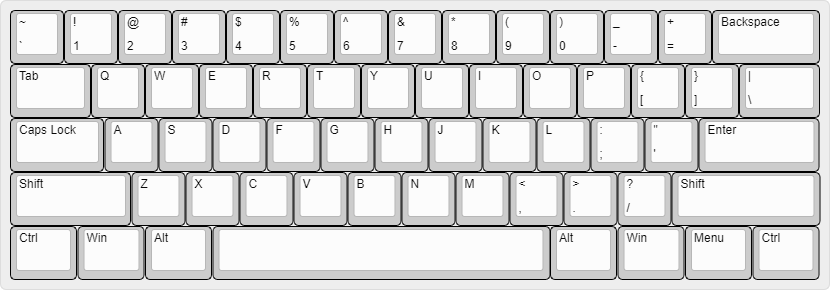
\includegraphics[width=.9\linewidth]{./images/base.png}
\end{center}

This is the ANSI 104 key layout with the function keys and right side of the keyboard (arrow keys, number pad, etc.) removed to save space. This physical layout is very common in the English-speaking world, and will be the one used in all discussions of key placement from here forward.

\begin{center}
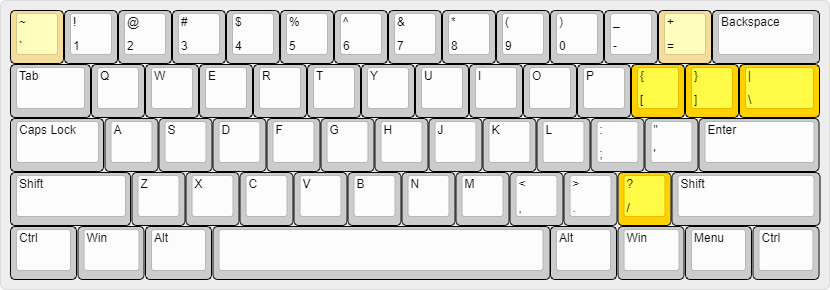
\includegraphics[width=.9\linewidth]{./images/unused-no-shift.png}
\end{center}

This image highlights unused punctuation keys that do not require shift. Numbers are ignored so that they may typed regularly if wished (and to stay consistent across languages). Note that the semicolon is ignored here as well, for the moment, since it is "used" as the Greek question mark. We'll return to it later. The apostrophe and hyphen both have uses (as a marker of elision and as an affix marker, respectively), so they have been excluded as well.

The two keys on the number row have been highlighted in a paler color, to indicate their relatively less favorable position. Keys on the number row require a great deal of hand movement to access, which makes them slower to type (see section §3.1.3).

\begin{center}
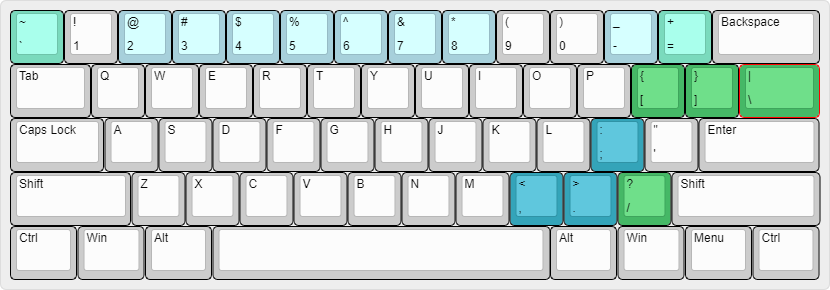
\includegraphics[width=.9\linewidth]{./images/unused-shift.png}
\end{center}

Finally, this image highlights the unused punctuation that do require shift. These keys are strictly inferior to those that do not (i.e., those from the above picture) since they require a whole additional keypress. Parentheses have been excluded since they are commonly used when writing ancient Greek (even if they do not show up in ancient sources), and the exclamation mark has also been excluded since it is not uncommonly used with imperatives.

Keys that have unused punctuation in both their unshifted and shifted states are shown in green, while those that only have unused punctuation in their shifted state are shown in blue. The shading distinction has been kept: the paler keys on the number row still indicate a relatively less favorable position. All of these keys are options that we can use for our diacritics here, and other things like punctuation below.

\subsubsection{Breathings}
\label{sec:org0eb6dd9}

Ancient Greek makes use of smooth breathing and rough breathing, and the diacritics in Greek look very similar to each other, except for a reversal of direction. Breathings are incredibly common in Greek, and thus it would be best if they did not end up on punctuation keys requiring shift or punctuation keys on the number row.

Visually, square brackets look similar to the breathings (not as similar as parentheses, but we can't use those), and since they do not require shift, they are easier to access than the other matched pair of characters we could use: < and >. Therefore, the breathings for this keyboard layout are placed on the square brackets: rough breathing on [, and smooth breathing ], as would be expected visually.

Along with vowels, the breathings may be put on rho.

\subsubsection{Accents}
\label{sec:org683d613}

\begin{itemize}
\item acute, grave, circumflex
\end{itemize}

\subsubsection{Iota subscripts}
\label{sec:org87fa469}

\subsubsection{Diaeresis}
\label{sec:org2194f01}

\subsubsection{The koronis}
\label{sec:orgbadb934}

\subsection{Additional markup}
\label{sec:orgcf2cd73}

\subsubsection{Vowel quantity: macrons and breves}
\label{sec:orgc0782b8}

\subsubsection{The underdot}
\label{sec:orgdceba13}

\subsection{Punctuation; language-specific symbols}
\label{sec:org4a93f89}

\subsubsection{Question marks and semicolons}
\label{sec:org6dbeb2f}

\subsubsection{A discussion of "hybrid" punctuation, and accessing normal punctuation when desired}
\label{sec:orgc31535c}

\{Todo: \footnote{Metrical marks, special numerals, drachma symbol}\}

\section{Section 5: Efficient typing practice for non-native languages}
\label{sec:org794dba7}

\subsection{Introduction to efficient typing}
\label{sec:org7584e51}

\subsubsection{Practicing based on word frequency}
\label{sec:orgc48b633}

\subsubsection{Practicing based on N-gram frequency; affixes}
\label{sec:org01cca89}

\begin{itemize}
\item (Derivational) Morphemes rather than words as a training focus
\end{itemize}

\subsubsection{Abbreviating very frequent words and phrases}
\label{sec:orge985f7c}

\subsubsection{Practicing the sorts of texts you are going to type}
\label{sec:orgc17d377}

\subsection{Creating necessary resources}
\label{sec:orga5708bc}

\subsubsection{Word frequency tables}
\label{sec:org85cab90}

\begin{itemize}
\item Perseus, TLG, handling overlapping forms
\end{itemize}

\subsubsection{N-gram frequency tables}
\label{sec:org93788b8}

\begin{itemize}
\item Similar process. Handling semantic boundaries in regexes? How to automate morphological analysis without obvious delimiters like spaces for words?
\end{itemize}

\subsubsection{Area-specific practice texts}
\label{sec:org7f17a68}

\begin{itemize}
\item Downloading from free/uncopyrighted sources. Perseus, Project Gutenberg.\footnote{Automate with script? Probably also outside scope of project.}
\end{itemize}

\subsection{Typing practice}
\label{sec:org87a55bf}

\subsubsection{Amphetype}
\label{sec:org0d5e86b}

\subsubsection{Lesson generation from frequency tables and practice texts}
\label{sec:orgbcde1bc}

\subsection{Crossover benefits}
\label{sec:orgc07b65d}

\subsubsection{Vocabulary lists by frequency for specific domains}
\label{sec:org306fb4e}

\subsubsection{Morphological analysis and generative vocabulary}
\label{sec:org4b6b83c}

\begin{itemize}
\item Prefixes, suffixes, and roots. Developing an eye for picking up meanings automatically, simply by knowing what different parts of the word mean in general.
\end{itemize}

\section{Section 6: Pedagogical applications}
\label{sec:org9be43ac}

\subsection{Orthography for digital natives}
\label{sec:org1d25c83}

\subsubsection{Standardization of letterforms}
\label{sec:org984b595}

\begin{itemize}
\item Reducing the learning load in the first few weeks of Hebrew: block scripts and cursive scripts.
\item Possible in handwritten as well (just only writing in block)
\end{itemize}

\subsubsection{Typing speed and writing speed}
\label{sec:org7d37a19}

\subsubsection{But the permanence of handwriting}
\label{sec:org686e75b}

\begin{itemize}
\item Tests
\end{itemize}

\subsection{Examples of typing-related pedagogical aids for Greek}
\label{sec:orgaff0b84}

\subsubsection{Learning the accentuation system}
\label{sec:org1f735b2}

\begin{itemize}
\item Practicing the typing of accents while learning about the rule of contonation, morae, and recessive accents.
\end{itemize}

\subsubsection{Common irregular verbs}
\label{sec:org2cd60a5}

\begin{itemize}
\item Practicing the typing of certain very common irregular verbs (like \emph{eimi}, e.g.) while simultaneously learning their paradigms.
\end{itemize}

\subsubsection{Practicing reading/speaking Greek; "reading by typing"}
\label{sec:org506a70c}

\begin{itemize}
\item Practicing typing in general by pulling in Greek texts from Perseus as typing training material. Students could be encouraged to also read the texts out loud as they type them. (Not necessarily understanding the Greek, but getting to see how it sounds and flows).
\end{itemize}

\section{Section 7: Concluding remarks}
\label{sec:org501a7a2}

\subsection{Specific implementation benefits}
\label{sec:org43856be}

\subsubsection{Who should make the switch to this system? Is this project really worthwhile?}
\label{sec:org35efcfc}

\subsubsection{The low opportunity cost for the next generation}
\label{sec:org025c896}

\subsection{Moving forward with more languages}
\label{sec:org18370d4}

\subsubsection{Current project: focus on Greek with Hebrew as a foil}
\label{sec:org11307fd}

\subsubsection{Possibility to expand much further}
\label{sec:org2537612}

\subsection{Suggestions for further research}
\label{sec:orgbb30185}

\subsubsection{Corpus generation}
\label{sec:org7542443}

\subsubsection{Morphological analysis}
\label{sec:org5913fef}

\subsubsection{Graphical frontends for customization}
\label{sec:org47272d9}

\subsubsection{System APIs for keystream manipulations \emph{across platforms}}
\label{sec:org69d3617}

\subsubsection{AI autograders for language exercises}
\label{sec:orgd7c37a0}



\section{Works Cited}
\label{sec:org6ab9119}

Chen Liao \& Pilsung Choe (2013) Chinese Keyboard Layout Design Based on Polyphone Disambiguation and a Genetic Algorithm, International Journal of Human–Computer Interaction, 29:6, 391-403, DOI: 10.1080/10447318.2013.777827 \\

Malas, Tareq M., Sinan Taifour and Gheith A. Abandah. “Toward Optimal Arabic Keyboard Layout Using Genetic Algorithm.” (2008). \\

Knisbacher, Jeffry M., and \texthebrew{הכתב העברי}, "DESIGN CONSIDERATIONS IN THE USE OF HEBREW AND OTHER NON-ROMAN SCRIPTS ON IBM-COMPATIBLE COMPUTERS." Proceedings of the World Congress of Jewish Studies (1989): 61-68. \url{http://www.jstor.org/stable/23535305}. \\

Deemer, Selden. "REPORT ON THE ARABIC LANGUAGE IN COMPUTERS SYMPOSIUM." MELA Notes, no. 23 (1981): 11-13. \url{http://www.jstor.org/stable/29785130}. \\

Mastronarde, Donald. "Before and After Unicode: Working with Polytonic Greek." Montreal APA Unicode Presentation, 2008. \\

Dhakal, V., Feit, A., Kristensson, P.O. and Oulasvirta, A. 2018. 'Observations on typing from 136 million keystrokes.' In Proceedings of the 36th ACM Conference on Human Factors in Computing Systems (CHI 2018). ACM Press. \\

Feit, Anna \& Weir, Daryl \& Oulasvirta, Antti. (2016). How We Type: Movement Strategies and Performance in Everyday Typing. 4262-4273. 10.1145/2858036.2858233. \\

E. Rumelhart, David \& Norman, Donald. (1982). Simulating a Skilled Typist: A Study of Skilled Cognitive-Motor Performance. Cognitive Science. 6. 1-36. 10.1016/S0364-0213(82)80004-9. \\

Allen, W. Sidney. 1999. Vox Graeca: a guide to the pronunciation of classical Greek. Cambridge [Cambridgeshire]: Cambridge University Press. \\

Verbrugghe, Gerald P. "Transliteration or Transcription of Greek." The Classical World 92, no. 6 (1999): 499-511. \url{doi:10.2307/4352343}.
\end{document}
